Before discussing the experiments conducted in this work, it is important to understand in which context the final model will be used to process experimental data. As well as the limitations of the model and the experimental setup.

\section{Detection and measurement algorithm}
\label{sec:algorithm}

The measurement process consists of several steps, each employing different techniques to improve measurement accuracy and reduce computation time.

\paragraph{Step 1: Image preprocessing} is done on the raw image data. This step is done to improve visibility of the droplets in the image and make a first guess as to which images actually contain droplets. 
The preprocessing is done batched by calculating the mean image $\mathbf{m}\in\mathbb{R}^{H\times W}$ as well as the mean greyscale value $\mu\in\mathbb{R}$ of the batch $\mathbf{B}\in\mathbb{R}^{N\times H\times W}$, subtracting $\mathbf{m}$ from each image in the batch, adding $\mu$ to each pixel and then mapping the resulting values to the interval $[0,255]$.
This process must be done batched because of memory constraints, but batching the images also has the advantage that images in one batch are more likely to be similar to each other in terms of lighting conditions, which makes the output more consistent.
This only applies if the images are taken in one measurement run.

The mean image subtraction is done to remove camera and lens artifacts such as hot pixels or dust from the images.
This is not primarily done to improve the models detection accuracy, but in order to filter out images that are not suitable for further processing.
The metric for deciding if an image contains any structure that could be a droplet is the \emph{Michelson contrast}, which is defined as 
$$
    C = \frac{I_\text{max}-I_\text{min}}{I_\text{max}+I_\text{min}},
$$
where $I_\text{max}$ and $I_\text{min}$ are the maximum and minimum luminance values in the image.
Since droplets have very dark and very bright regions, they produce a high Michelson contrast.
Images aren't considered for further processing if $C$ is below a certain threshold.
The reason artifacts need to be removed is that the they are very dark compared to the background, which means even images without any droplet structures will have a high Michelson contrast.

Lastly, before applying the model to the images, they are normalized to have a mean of 0 and a standard deviation of 1 using ImageNet mean and standard deviation to match the training augmentations.

\paragraph{Step 2: Droplet detection} is done by a model trained to identify droplets with dark borders and bright centers as in-focus and segment the images into three classes, \emph{droplet border}, \emph{droplet inside} and \emph{background}.
Segmenting the images into three classes instead of two is important in the next step, since it helps to detect errors the model made in the segmentation process.

Details on model training and evaluation can be found in section \ref{sec:experiments}.

\paragraph{Step 3: Droplet measurement} is done by first grouping all adjacent pixels labeled as \emph{droplet border} in the segmented image to distinct instances. 
This is essentially done by choosing a starting pixel with the correct label and scanning its neighboring pixels to find all pixels that are also labeled as \emph{droplet border}.
This step is repeated for this new set of pixels until no more pixels with the correct label can be found.
The process starts again for a new pixel that has not been assigned to a droplet yet, until all labeled pixels have been precessed.
The library \emph{scikit-image}\cite{waltScikitimageImageProcessing2014} is used to do this which employs several tricks to speed up this process \cite{wuOptimizingConnectedComponent2005}. 

As a first filtering step, all areas that are smaller than a certain threshold are now discarded, since no droplets below a certain size can be expected to fit the criteria for being in focus.
For each remaining area, the locations of all pixels is averaged to locate the center of the droplet.
Since the droplet is approximately circular, the average distance of all pixels from the center is calculated and used as a measure for the radius of the droplet.
Because the border of the droplet has a certain width and labels sometimes extend beyond the actual droplet, only the values between the 80th and 95th percentile of the distances are used to calculate the radius.

\section{Common problems and limitations}
\label{sec:limitations}

The model used to segment the image is not perfect, which means that sometimes areas which do not belong to a droplet are labeled as \emph{droplet border} or \emph{droplet inside} or the model fails to detect a droplet that is actually present in the image.
In this section, the most common errors are discussed and possible solutions are proposed, some of which are implemented already.

\paragraph{The model labels an out of focus droplet or other noise partially with border and center labels.}
\label{sec:partially_wrong}
This is the most common error observed when applying the model to experimental data examples for which can be seen in \ref{fig:partially_wrong}.
The model will assign a border label to the dark pixels of an out of focus droplet or a center label to brighter areas of the image that are not part of a droplet, possibly even both for the same structure.
However, this will very rarely happen in a way in which the border region completely surrounds the center region in a closed shape, which can be used to filter out these errors.

\begin{figure}[htbp]
    \centering
    \begin{tabular}{ll}
        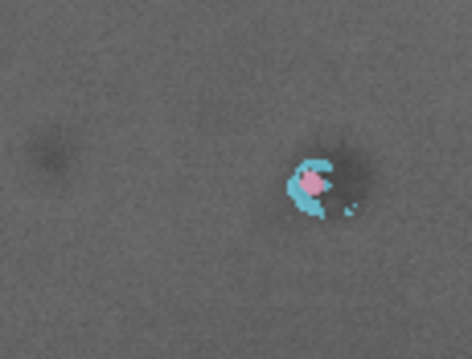
\includegraphics[width=0.4\textwidth]{images/bad1.png}
        &
        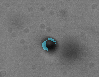
\includegraphics[width=0.35\textwidth]{images/bad2.png}
    \end{tabular}
    \caption{Example images showing a labeling error as described in section \ref{sec:partially_wrong}. Blue pixels represent \emph{droplet border} labels, and pink pixels represent \emph{droplet inside} labels.}
    \label{fig:partially_wrong}
\end{figure}

Training the model to assign two different labels for the droplets instead of one allows the criterion of droplets having a closed border around a center region to be used not only during training, but also after segmentation.
To check if a border area such as the ones described in Figure~\ref{sec:algorithm} fulfills this criterion, the algorithm calculates its \emph{alpha shape}\cite{edelsbrunnerShapeSetPoints1983a} and then checks if any of the pixels inside the shape are labeled as \emph{droplet inside}.

The alpha shape of a set of points is a generalization of their \emph{convex hull} and for a real number $\alpha$ includes all edges between the points for which a \emph{generalized disk} with radius $\frac{1}{\alpha}$ can be drawn so that the points of the edge lie on its border and the disk contains no other points. For $\alpha=0$, the generalized disk becomes a half-plane and the alpha shape is equivalent to the convex hull. In the code, the alpha shape is calculated using the \emph{alphashape}\cite{bellockBellockkAlphashapeV12021} package, which first calculates the \emph{Delaunay triangulation} of the points and then uses the criterion described above to determine which edges to include in the shape. The parameter $\alpha = 1$ is used since the pixel coordinates are discrete and the pixels are directly adjacent to each other. 

This method of filtering works very well for any but the most extreme cases and improves the accuracy of the measuring process significantly.

\paragraph{The model labels an out of focus droplet or other noise completely with border and center labels.}

This is a much rarer error than the one described in the previous paragraph, but it can still happen. 
It is mostly encountered when the image is very dark overall, which ironically causes the preprocessing step described in \ref{sec:algorithm} to produce bright artifacts in such images, instead of removing dark spots. 
One example of such an image can be seen in Figure~\ref{fig:totally_wrong_a}.
Since identifies in focus droplets by their bright center, this behaviour is not completely unexpected.

However, very rarely the model will assign a false positive even to an area which is not significantly brighter than the background, as can be seen in Figure~\ref{fig:totally_wrong_b}.

\begin{figure}[htbp]
    \centering
    \begin{subfigure}{\textwidth}
        \makebox[\textwidth][c]{
            \begin{tabular}{ll}
                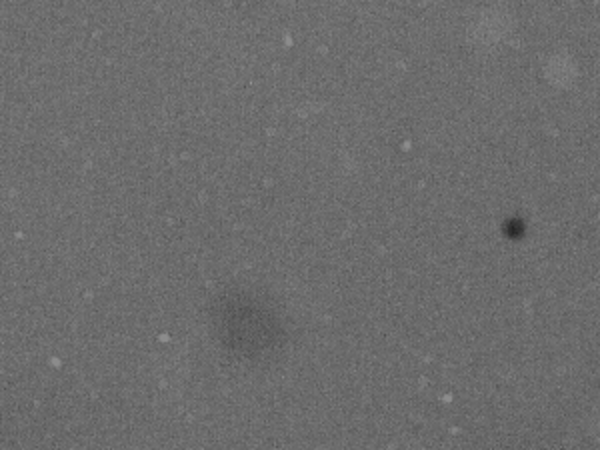
\includegraphics[width=0.45\textwidth]{images/bad4_pic.png}
                &
                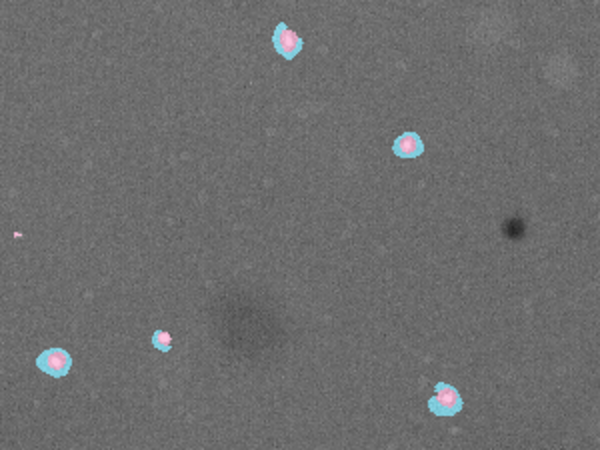
\includegraphics[width=0.45\textwidth]{images/bad4_mask.png}
            \end{tabular}
        }
        \caption{The model identifying bright artifacts in dark images as droplets. Note that only bottom left and top right labels are fully closed shapes, which can't be filtered out.}
        \label{fig:totally_wrong_a}
    \end{subfigure}
    \begin{subfigure}{\textwidth}
        \makebox[\textwidth][c]{
            \begin{tabular}{ll}
                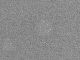
\includegraphics[width=0.45\textwidth]{images/bad3_pic.png}
                &
                
\includegraphics[width=0.45\textwidth]{images/bad3_mask.png}
            \end{tabular}
        }
        \caption{The model indentifying a comparatively brighter spot as a droplet.}
        \label{fig:totally_wrong_b}
    \end{subfigure}
    \vspace{0.2cm}
    \caption{Examples for cases where the model confidently labels an out of focus droplet or other noise completely with border and center labels. The left image shows the original image, the right image shows the segmentation mask. Blue pixels represent \emph{droplet border} labels, and pink pixels represent \emph{droplet inside} labels.}
    \label{fig:totally_wrong}
\end{figure}

This kind of error is much more severe, since there aren't any criteria to differentiate these kinds of false positives from the structure of the actual droplet labels.
Thus, the only way to mitigate this that comes to mind are improving image preprocessing and/or training the model differently to not make these kinds of mistakes.

One idea to improve the preprocessing is to use a different technique for removing the artifacts. 
The current method of removing the artifacts by subtracting the background image from the original image is very simple and works well if the images in the batch are similar in brightness, but it is not very robust to outliers.
A different approach then, would be to use the background image as a mask for identifying artifact locations instead, and overwrite the pixels in the original image with a more appropriate value. 
This could either be the mean brightness of each individual image, or the values at the same pixel location in the original image with a gaussian blur applied to it.
A process like this could help in minimizing bright artifacts, which seem to be the main cause of this kind of error.
For this, \emph{inpainting methods} \cite{OpenCVImageInpainting,teleaImageInpaintingTechnique2004,bertalmioNavierstokesFluidDynamics2001} could do a good job, however they were found to be too computationally expensive for the task at hand.

To instead make the model more robust to these kinds of artifacts, some kind of data augmentation could be used that mimics the effect of the artifacts, such as \emph{salt-and-pepper/binary noise}. Another option would be to explicitly use additional samples of images the model seems to find difficult to classify correctly, such as the ones shown in Figure~\ref{fig:totally_wrong}. These examples would need to be labeled of course, but could potentially improve the model substantially in this regard.

\paragraph{Very fast droplets} that travel a significant distance in the time it takes to expose the image (inv. proportional to \emph{shutter speed}) appear as streaks instead of circles. 
Since the model is trained to identify droplets that are ellipsoidal in shape, it won't be able to label those streaks correctly.
The shape of these streaks is also much less distinct than the shape of the droplets, which makes it harder to say if the streak is in focus or not.

Up to a point, this can be mitigated by increasing the shutter speed during image capturing, however this will also decrease the amount of light that reaches the camera, making the images darker overall, so depending on the lighting conditions, this may not be a viable option.

Using a different model that is trained to identify streaks instead of circles or even training the same model to segment streaks into a different class could be a solution to this problem. 

Doing this could have some additional benefits.
For example, by finding the minimum angled rectangle that contains the streak we could calculate the ratio of the width and height of the rectangle to estimate the speed of the droplet, since the shutter speed is a known parameter and the longer side of the rectangle corresponds to the distance the droplet traveled in the time it took to expose the image.
Since the speed of the droplet is another interesting parameter to measure, this could be a useful addition to the model.
One might even be able to deliberately lower the shutter speed to make the droplets appear as streaks for the purpose of measuring the distribution of the droplet velocity.

Due to time constraints, this idea couldn't be explored further in this thesis, but could be an interesting topic for future work.

\paragraph{Droplets that are too small} are not reliably identified by the model, since the smaller the droplet, the less distinguishable the different parts of the droplet become. 
This is an inherent problem of techniques using imaging as a measurement method, since there is always a limit to the scale at which objects can be resolved.

Up to a point this can still be mitigated by increasing the resolution of the camera or the magnification of the lens, but this will also increase the cost of the setup and will only be possible to a certain extent.

Since this problem isn't something that is specific to the algorithm, but rather a limitation of the imaging technique itself, there isn't much that can be done to improve the model in this regard.
For the actual usage of the technique, this means human oversight is still necessary for deciding if the approach is applicable to specific set of captured data.

\paragraph{In focus criteria may be unrepresentative of actual in focus droplets.} Instead of an error observed in the measuring process, this is a potential problem with the method itself.
Which droplets are considered in focus and should be included in the measurement is a key aspect of the process, since data has to be labeled accordingly. Structures with extremely sharp corners are exceedingly rare in the data captured by the experimental setup, which is why \Citeauthor{kapplAkustischInduzierteVernebelung2022}\cite{kapplAkustischInduzierteVernebelung2022} argues that structures with a dark border and a bright center should be considered sufficiently in focus.

The reasoning behind this is that light that passes through the outer areas of the droplet is scattered more strongly, resulting in less light reaching the camera, while light that passes through the center of the droplet passes through straight, with beams near the center even being focused slightly.

The success of the method as a measurement technique depends heavily on the veracity of this assumption. 
However, if in the future, other criterions are found to be more suitable to differentiate between in focus and out of focus droplets, the method could theoretically be adapted to use those instead.